\chapter{Analyses}

\label{ch:analysis}

Before designing an educational product, it is important that the designer first acquaints himself with the extrinsic factors important to this product. In order to discover the important characteristics of these factors, \citeA{instructionaldesign} enlist three types of analyses to be conducted, together with steps for conducting them. These are an analysis of the context, of the learner, and of the learning task. Although these analyses are more targeted towards instructional design, and therefore more focused on a specific group being taught specific content, these analyses still provide relevant information for the design choices and the evaluation. However, the steps are adjusted and generalised or even omitted in order to fit the design of the more generic learning tool. The information gathered in order to conduct these analyses mainly stems from meetings with one of the teachers. This might not be the most reliable source of information because of the lack of triangulation, and should therefore not be taken as insight in the curriculum of Dutch Literature courses in secondary education, but rather as context information relevant to the design. The most important findings are described within this chapter, along with their implications for the design of the software.

\section{Analysis of the learning context}
\label{sec:contextanalysis}

As already stated in the \nameref{sec:intro_evaluation} section on page~\pageref{sec:intro_evaluation}, the evaluation of the flashmap system will be evaluated within the Dutch secondary school Stedelijk Lyceum, with students having to learn about the Renaissance genres in Dutch Literature. Although the general needs for a flashmap system are shortly provided within the \nameref{sec:intro_evaluation} on page~\pageref{sec:intro_evaluation}, it is still important to investigate the specific needs of the context where the programm will be implemented. Therefore, this context will be further investigated within this section, starting with the Needs Assessment \cite{instructionaldesign}. 

\subsection{Needs assessment}
\label{subsec:needsassessment}

There are multiple reason why teachers think it is important to learn about Dutch renaissance literature: one could argue that this way the knowledge is passed onto a new generation, keeping it relevant; understanding the history of literature is important for understanding modern literature; and literature can provide certain insights to the individual reading it \cite{opinion1, opinion2}. Furthermore, the school is extrinsically motivated to teach the subject matter, since subdomain E2 and E3 within the Dutch national exam programm state that a student has to recognise and distinct between literary text genres, apply literary concepts in the interpretation of literary work, provide the outlines of the literature history, and place literary works in this historical perspective.

The teacher did confirm the need for better retention and comprehension of the content already stated within the \nameref{ch:problem}, since she indicated that most of the time the students only learned the night before the exam in order to get a high (enough) grade and consequently forget everything again. Both using a flashcard system and the flashmap system should accomodate this need. Furthermore, she deemed them to become more familiar with the Dutch Renaissance writers or work to be the most important, entailing that students recognise impotant names or that they can distinguish between different genres. Based on these statements, the goals within the context are in line with students memorising and understanding all of the facts, without them being too ambitious. Finally, the teacher provided a test from the previous year to offer some more concrete examples of what she wanted the students to know, of which an English translation is included in the appendix on page~\pageref{app:exampletest}. From this test, more goals can be extrapolated, such as students having to not only distinguish different genres, but also having to define them or provide characteristics, and recognise the application of these features in both examples of the time periods as well as modern examples. Furthermore, they have to be able to relate the famous writers and writings to the genres.

\subsection{The learning environment}
\label{subsec:learningenvironment}

The Stedelijk Lyceum is an open denominated school organisation, consisting of 7 schools on different locations. The school approached within this project has been approved by the Dutch Inspection of Education \cite{inspectierapport}. The course on Dutch renaissance literature consists of two different types of learning activities, which are classroom instruction, and individual learning at home by the students. There are two sessions of classroom instruction, both lasting 50 minutes, in which the 100 students are divided over the three teachers in static groups on separate locations. These lessons take place over the course of two weeks, with one lesson provided in one week. Within these lessons, the teachers transfer knowledge and provide excersises for the students. Outside of the lessons, the students still have to study the textbook Laagland individually \cite{laagland}, which contains all of the materials which will be prompted on a final written assessment. As already stated before, the teacher indicated this activity mostly to take place on the evening before the assessment, and only on a superficial level. Finally, this assessment takes place in the second week after the final instruction, and will be similar to the example test included in the appendix on page~\pageref{app:exampletest}.

The teacher stated that the course mainly consisted of the rote memorisation of facts, and that she was still doubtful whether the students would actually be willing to participate in the evaluation of the Flashmap system. Yet, she did see the general use of the tool for achieving the learning goals, and therefore still seemed to be enthusiastic in cooperation and encouraging the students to participate. The only two technical problems are that there is not too much time for extra activities within the lesson plan and the teachers being quite busy themselves, and that the technological possibilities within the classroom are limited. Within the classroom, only a couple of computers are available for use, and still run relatively old software. Therefore, the activities envolved in using the flashmap have to target the individual learning of students, since they have more time outside of the lesson plan, and mostly do possess the hardware and software necessary to run the software.

\section{Analysis of the learner}
\label{sec:learneranalysis}

\subsection{Physiological characteristics}

The physiological characteristics of the respondent's brain provide important implications for the design of the software. They are enrolled in grade 4 of Dutch secondary education, and therefore should be around the age of 16-17, with some deviations due to students either having skipped or repeated a grade. Therefore, the students are generally considered to be either at the end of puberty, or the beginning of young adolescence. The \nameref{ch:theory} chapter on page~\pageref{ch:theory} already provides general theories about the learning process within the brain. However, during late puberty and early adolesence, the brain is still heavily in development, especially the prefrontal cortex. \cite{blakemore}. In order to map out the changes in the adolescent brain, \citeA{giedd} performed a longitudinal MRI study of the brain development during this period, where three themes emerged within the adolescent development of the brain:

\begin{enumerate}
    \item After a peak in growth of both brain cells, connections and neurotransmitters during childhood, one can see a decline in adolescence;
    \item The connectivity between different regions of the brain increases;
    \item A new balance is formed among frontal and limbic lobes.
\end{enumerate}

The first theme is a result for the brain becoming more streamlined after having collected a lot of information during late childhood, making it more efficient (see also \nameref{subsec:interferencedecay} on page~\pageref{subsec:interferencedecay}). This is also known as peak plasticity, after which a decrease can be observed. \citeA{powell} describes this phenomenon as \emph{Use it or lose it}, since the brain rigorously selects the specific memories which are activated during this time. The second theme refers to the strengthening of specific memories, which are enhanced during that period. Here the flashcard system proves to be a useful tool, since it focuses on repeating specific associated pairs that the learner wants to remember.

Finally, during adolescence a shift is made from ``cold'' to ``hot'' cognition, where the former relates to hypothetical, low-emotion reactions, and the latter to high arousal decision making, strongly influenced by peer pressure and real, direct consequences. This is highly related to the prefrontal cortex being heavily developed, resulting in the teenage brain to rely more on the amygdala which is the more emotional, impulsive area of the brain. This means that for students to be motivated to learn, they either need a strong intrinsic motivator, or they have to rely on what \citeA{powell} describes as an ``external prefrontal cortex'', which can be either a reward or a person reminding them to study (e.g. the teacher or a parent). Therefore, extrinsic factors such as the usefulness of the system to passing the school test, a voucher for icecream, and the teacher are used to motivate the students to use the system.

\subsection{Cognitive characteristics}

All students should have learned about the relevant time period in their history classes prior to this course (e.g. the Spanish War, the Lutheran reformation etc.), providing the relevant knowledge to understand the context of Dutch renaissance literature. Additionally, the students have received a similar instruction on Dutch medieval literature, which is also relvant for concepts in the renaissance literature, such as the \emph{Mecenas}, the \emph{Lyriek} and \emph{Rederijkers}. Therefore, these concepts form the root concepts from which to start within the concept map.

However, one difference between students is whether they chose technical or society-related subjects. This makes up for different specific aptitudes within this specific Dutch literature course. Furthermore, some of the students are also enrolled in classical subjects, and because the Dutch renaissance literature has a lot of connections with classical genres, these students might have an advantage in prior knowledge. Both technical and society-oriented profiles, and classical and non-classical profiles are therefore accommodated for within the concept map.

\subsection{Social characteristics}

Among other data, the CBS offers descriptives of students, categorised per national district. This descriptive data entails information about the age, sex, type of education, and ethnicity of students, and the interactions among these variables \cite{cbsethn}. From this data, descriptives about 16-17 year old students from Enschede enrolled in vwo grade 3-6 was extracted, displaying their age and ethnicities. 23\% of the 16-17 year old students are enrolled in VWO, where 44\% is male and 56\% is female. The distribution of ethnicity is visualised in figure~\ref{fig:ethnicitychart}. 77\% of the students are native and 31\% are non-native. 9\% of the students is western non-native, and 22\% is non-western non-native. The CBS defines a non-western non-native is an non-native originating from Afrika, Latin-Amerika and Asia (except for Indonesia and Japan) or Turkey. The most prevalent non-western ethnicity is Turkish, with 8\%.

\citeA{grever} provide information on the perspectives on learning history by Dutch, English and French high school students. Within this study, students were asked several questions about what kinds of history, which periods of history are important or interesting for the students, and what the meaning of history is for their personal lives and what they believe to be its relevance for society. For Dutch students, this study found that the history of ones own family generally ranks high, and after that the history of the country where the parents come from (both for natives and non-natives). This means that native students might be more interested in learning about the subject than non-native students. Furthermore, the history of ones own religion is mostly important for Moroccan and Turkish students (which are mostly muslim), so the history of christianity is generally not that interesting towards most students. The study also found that the time period of early modern history is the least interesting for students, no matter the gender or nationality, despite that in the Netherlands the most important topic is the rise of the Dutch republic and the Golden Age (the content of the subject used within this study). Finally, the study states that there were no significant differences in perceptions of pre-vocational students and HAVO/VWO students in these respects, although one might expect Gymnasium students to be more interested in the classical revival of art during the renaissance than the Atheneum students.

\begin{figure}
    \centering
    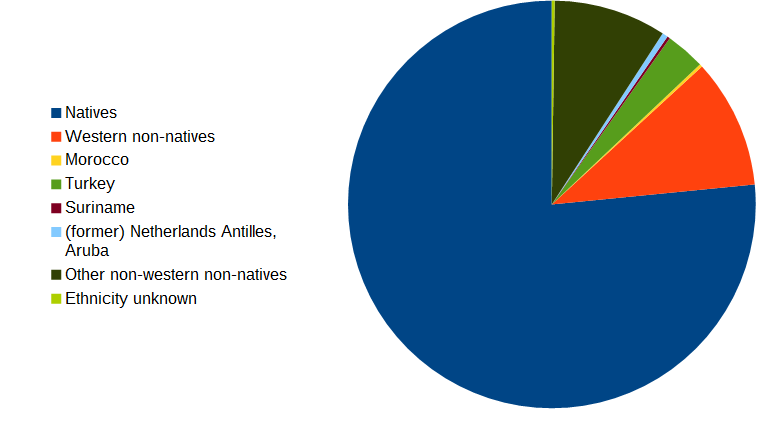
\includegraphics[width=0.7\textwidth]{img/ethnicitychart.png}
    \caption{The distribution of ethnicities among 16-17 year old vwo students of education type vwo3-6 \protect\cite{cbsethn}}
    \label{fig:ethnicitychart}
\end{figure}

Finally, the CBS also offers statistics about religious denominations \cite{cbsdenom}, which state that 57\% of the people in the province of Overijssel is affiliated to a church. These affiliations are split up in different religions: 22\% Roman-Catholic, 8\% Protestant, 12\% Dutch Reformed, 7\% Continental Reformed, 4\% Islam, and 5\% miscellaneous (see figure~\ref{fig:denominations}. 43\% is not affiliated to any church, however this does not necessarily entail that they do not have a religious worldview. Data is also offered on how frequent people visit the church: 14\% visits every week or more often, 4\% two or three times a month, 4\% once a month, 8\% less than once a month, and finally 70\% (almost) never (see figure~\ref{fig:churchvisits}. This would indicate that although there is a majority affiliated with a certain church, most of the people do not actively take part in their respective community. There are also more specific statistics available about the region of Twente only \cite{cbsdenomold}, however these are older and might already have changed significantly over the last 13 years. Yet, they state that Twente is more religious than the overal province of Overijssel. Unfortunately, there are no statistics available about Enschede only. Finally, the school of the target group has an open (i.e. non-religious) denomination, whereas the other large school in Enschede has a christian denomination, so one might expect mainly the students without any strong religious views to choose for this school. Still, since christianity is generally prevalent within the region, students are highly likely to be familiar with the christian themes relevant to understanding the literature from the renaissance period.

\begin{figure}
    \centering
    \begin{subfigure}[b]{0.7\textwidth}
        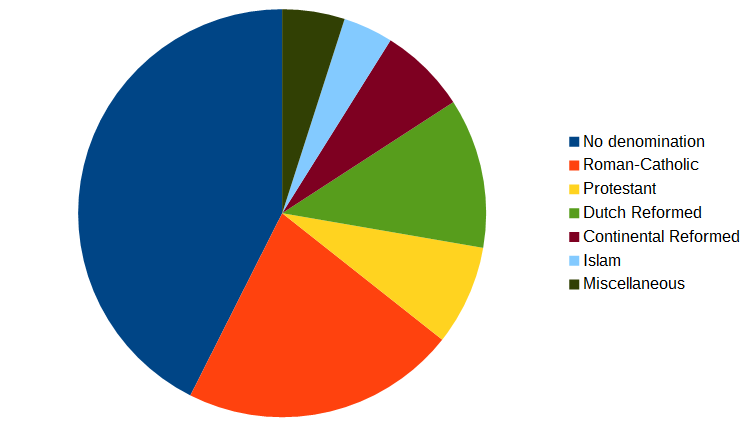
\includegraphics[width=\textwidth]{img/denominations.png}
        \begin{center}
            \caption{A distribution of church affiliations}
            \label{fig:denominations}
        \end{center}
    \end{subfigure}
    \begin{subfigure}[b]{0.7\textwidth}
        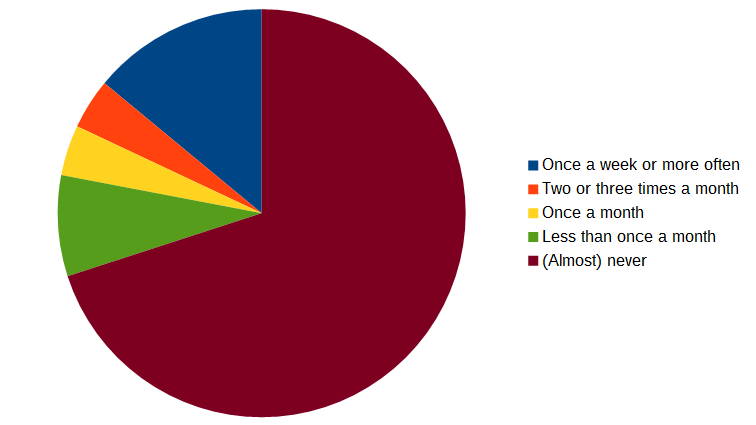
\includegraphics[width=\textwidth]{img/churchvisits.png}
        \begin{center}
            \caption{The distribution of frequencies of church visits within the group of people affiliated to a church}
            \label{fig:churchvisits}
        \end{center}
    \end{subfigure}
    \caption{Denominations within the region of Twente \protect\cite{cbsdenom}}
    \label{fig:religion}
\end{figure}

\section{Analysis of the task}
\label{sec:taskanalysis}

Finally, the characteristics of the task itself will be investigated in order to learn how to design a tool in such a way that it facilitates or augments the learning process. \citeA{instructionaldesign} enlist primary steps for performing a learning task analysis, which are writing a learning goal, determining the types of learning of the goal, conducting an information-processing analysis of that goal, conducting a prerequisite analysis and determining the type of learning of the prerequisites, writing the learning objectives for the learning goal and each of the prerequisites, and writing the test specifications. However, within this project the instruction has already been written \cite{laagland}, and only has to be used to create a concept map. Still, knowledge of the underlying structure of the instruction might prove to be helpful for finding the relevant elements, and it is also useful to investigate the specific uses of the instruction within the context of this project.

\subsection{Learning goals}

The direct learning goals of the instruction can be found in paragraph 13.4 of Laagland, the specific instruction for the Dutch renaissance literature, where the previous paragraphs only provide the prerequisite knowledge necessary to understand this paragraph. The different chapters describe the \emph{emblematiek}, the \emph{lyriek}, the sonnet, and the different theatrical genres (the tragedy, the comedy, and the \emph{klucht}). One of the goals of this instruction is that the students are able to describe these genres, and are able to differentiate between the subgenres or terminology within these genres. However, the students also have to be able to relate these genres to the general context described in the previous chapters, which consist out of the political, the socioeconomic, and the cultural backgrounds.

\subsection{Types of learning}

Attaining these skills are mainly intellectual in the typology defined by \citeA{instructionaldesign}, because the students mainly have to be able to describe and discriminate between defined concepts. However, there is also a certain amount of declarative knowledge learning involved because students have to first learn and memorise certain definitions or conceptual organisations. Furthermore, within the book there are not only abstract concepts being defined, but also declarative knowledge such as names of important authors (Vondel, Bredero etc.), books or plays (e.g. the \emph{Klucht van de koe}), and certain historic events such as the migration of calvinists from Antwerpen to Amsterdam in 1585.

\subsection{Concept map}

Because the information has already been defined within the textbook (both the new content and prerequisite content), the information-processing and prerequisite analysis activities have been replaced by translating the content of the instruction within the textbook to a concept map. Within this map, not only the relevant concepts, names and events are presented, but also the relations between them, providing a more meaningful representation. Furthermore, the concept map also contains information about the order in which the concepts have to be learned, because of the direction of the relations. The data used for the concept map is uploaded on github\footnote{\url{https://github.com/mcvdenk/MasterThesis-Software/blob/master/database/concept_map.json}}. A direct visualisation is too extensive to be feasibly included within this report, however a digital visualisation is available\footnote{\url{http://www.mvdenk.com/thesis/concept_map/}} (after a short initial rendering time due to its size). The \nameref{ch:client} chapter on page~\pageref{ch:client} will elaborate further on the design choices for the concept map. Finally, this map is directly shown to the students within the flashmap condition during the experiment.

\subsection{Flashcards}

The activity of specifying the learning objectives is replaced by formulating the flashcards, because the flashcards already form the specific knowledge-based learning objectives. They already contain the most important types of information which should be included in an objective, namely the statement of the terminal behaviour (the answer itself), the conditions of demonstration (given this question, the student can reproduce the correct associated answer). The standards or criteria for these objectives are globally defined, namely that the student has to be able to demonstrate that he knows the correct concept corresponding to a parent node and edge label. The flashcards are directly based on the previously defined concept map. Within this activity, edges and their corresponding parent nodes were transformed to a question, and the child node formed the answer to that question. For example, the nodes \emph{Strijdliteratuur} and \emph{Actualiteit}, respectively connected by the edge \emph{verwees naar}, is translated to a flashcard "Q: Waar verwees de Strijdliteratuur naar?" $\rightarrow$ "A: Naar de actualiteit" (\emph{Translation:} To which did the war literature refer? To actual events). Sometimes, multiple edges from one node to several child nodes having the same label or falling within the same category were translated to only one single flashcard. The data for the flashcards can be found again on github\footnote{\url{https://github.com/mcvdenk/MasterThesis-Software/blob/master/database/flashcards.json}}.

\subsection{Test specifications}

The assessments conducted before and after the students have used the learning tool consist partly out of the questions from the flashcards for measuring knowledge reproduction, but also partly of questions targeted to measure the comprehension levels of the students (see \citeNP{bloom}). On both assessments for all questions, the students are asked to fill in an answer in a textbox. In order to answer the questions for comprehension, a student has to be able to draw relations between not directly linked nodes, and thereby requires a higher degree of mastery of the content. It does however not yet contain any questions where students have to apply the content within different context, or have to think outside of the content directly taught, since these questions would rate on even higher levels on the taxonomy of Bloom. Finally, the questions are phrased according to the specified action verbs related to the level of learning. A more detailed elaboration of the test construction and analysis can be found in the \nameref{sec:instrumentation} section on page~\pageref{sec:instrumentation}, and all of the comprehension level questions are included on github\footnote{\url{https://github.com/mcvdenk/MasterThesis-Software/blob/master/database/itembank.json}}.
